\section{Pre processing}
\begin{figure}[ht]
    \centering
    \begin{subfigure}{0.4\linewidth}
        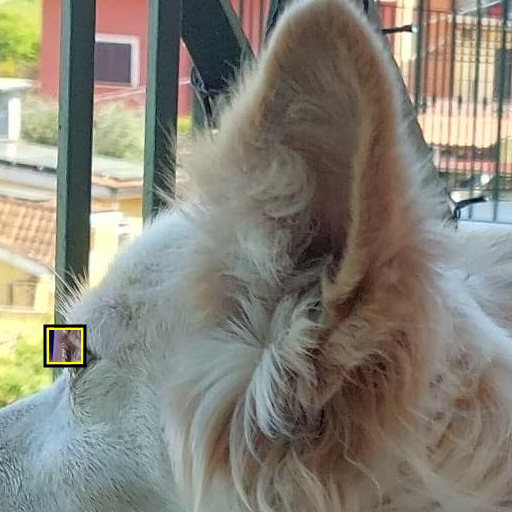
\includegraphics[width=\linewidth]{Figures/example_square.png}
    \end{subfigure}
    \hspace{2cm}
    \begin{subfigure}{0.4\linewidth}
        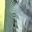
\includegraphics[width=\linewidth]{Figures/example_detail.png}
    \end{subfigure}
    \caption[Pixel grid detail]{Image detail.}
    \label{fig:example_detail}
\end{figure}
\begin{toReview}
%La digitalizzazione delle immagini è un passo fondamentale per preparare le opere d'arte alle analisi che verranno effettuate. Per comprendere appieno il funzionamento di queste trasformazioni, è importante acquisire una conoscenza approfondita del processo attraverso cui un'opera pittorica viene catturata da una macchina fotografica e successivamente digitalizzata in un dispositivo elettronico.
Digitising images is a fundamental step in preparing the data set for analysis. To fully understand how these transformations work, it is important to understand the process by which a work of art is captured by a camera and then digitised in an electronic device.

\paragraph{Definition of image: from the real world to the virtual world}
%Gli artisti dell'antichità utilizzavano varie tecniche, come la camera oscura e i principi della geometria proiettiva, per rappresentare i paesaggi in modo realistico. Durante il Rinascimento, hanno ulteriormente perfezionato questi metodi con strumenti come la camera lucida, mostrando una comprensione matematica avanzata in opere d'arte come la Scuola di Atene di Raffaello.\begin{toDo} citare fonte \end{toDo}.
Artists of antiquity used various techniques, such as the camera obscura and the principles of projective geometry, to represent landscapes realistically. During the Renaissance, they further refined these methods with tools such as the camera lucida, showing advanced mathematical understanding in works of art such as Raphael's School of Athens.\footnote{for more about camera obscura, see\newline\url{https://en.wikipedia.org/wiki/Camera_obscura}}

%\noindent L'invenzione della fotografia nel $1826$, in concomitanza con il movimento artistico del Realismo, segnò un momento fondamentale nella storia dell'arte visiva. La fotografia, con la sua capacità di rappresentare la realtà in modo oggettivo, divenne uno strumento sempre più utilizzato dagli artisti. L'avanzamento delle conoscenze in ottica e chimica portò alla creazione della fotografia analogica \begin{toDo} citare fonte e inserire immagine \end{toDo}.
\noindent The invention of photography in $1826$, in conjunction with the art movement of Realism, marked a fundamental moment in the history of visual art. Photography, with its ability to represent reality objectively, became a tool increasingly used by artists. The advancement of knowledge in optics and chemistry led to the creation of analogue photography.\footnote{for more about history of photography, see\newline\url{https://en.wikipedia.org/wiki/History_of_photography}}
\begin{figure}[ht]
    \centering
    \begin{subfigure}[t]{0.4\linewidth}
        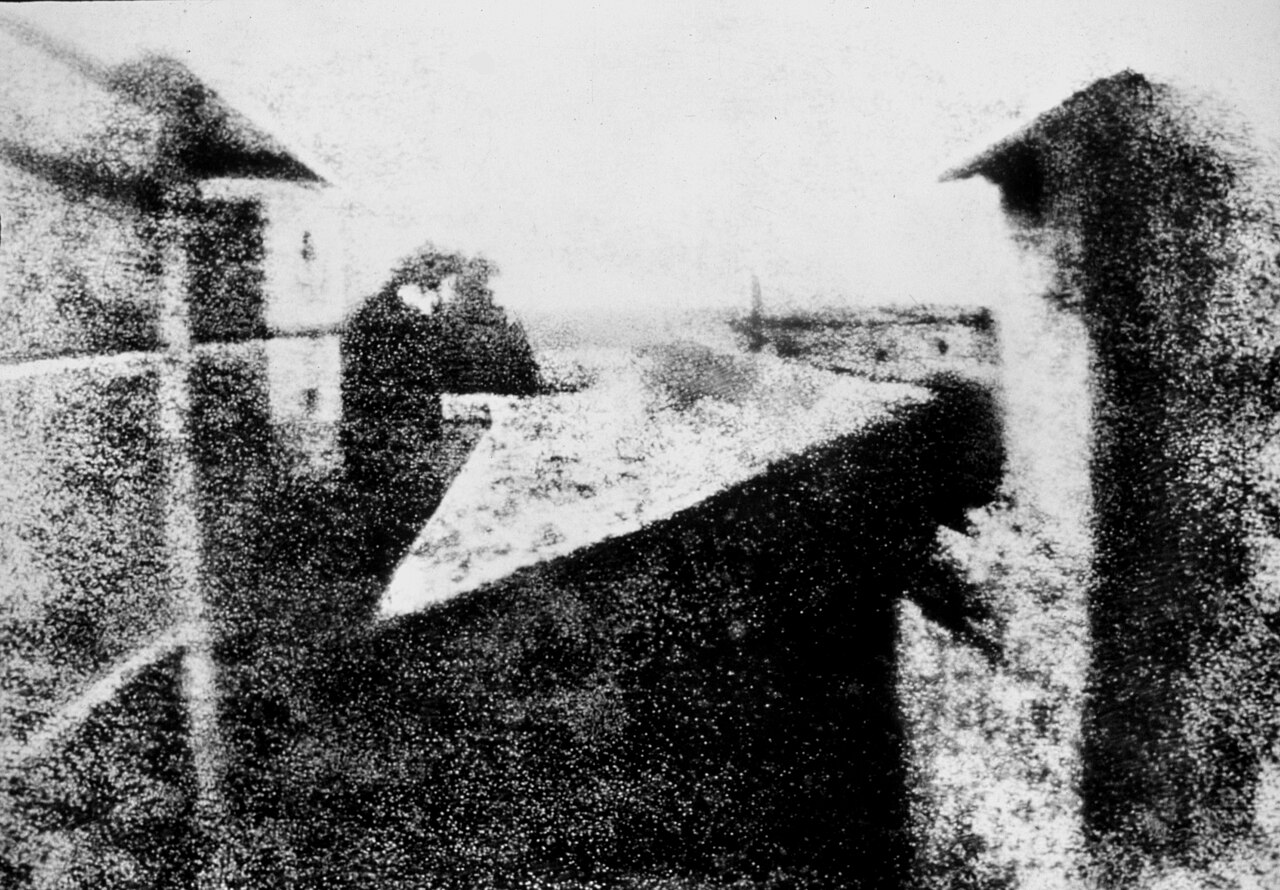
\includegraphics[width=\linewidth]{Figures/FotoStoria.jpg}
        \caption{'View from the Window at Le Gras', Joseph Nicéphore Niépce, c.1826, Heliography, Harry Ransom Center, University of Texas at Austin, USA\cite{FirstPhoto}.}
    \end{subfigure}
    \hspace{2cm}
    \begin{subfigure}[t]{0.4\linewidth}
        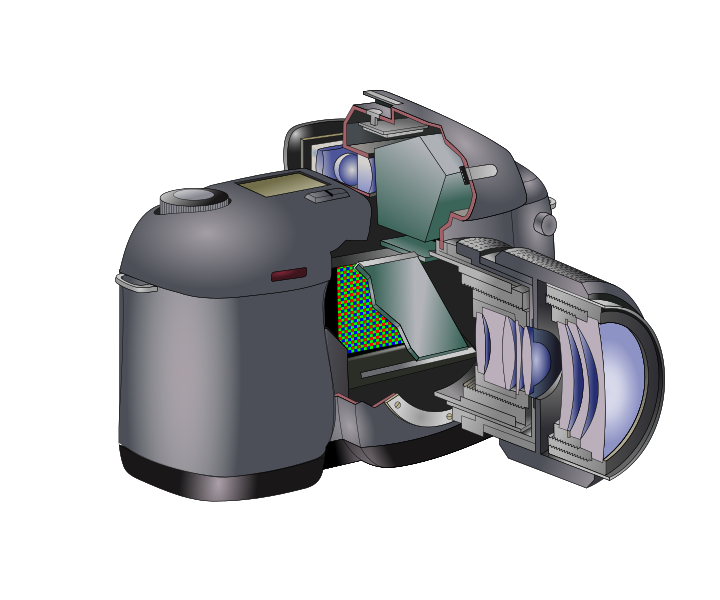
\includegraphics[width=\linewidth]{Figures/digitalcamera.png}
        \caption{Illustration of digital camera\cite{Reflex}.}
    \end{subfigure}
\end{figure}

%\noindent Nel corso degli anni ottanta, con l'avvento della tecnologia informatica, la fotografia digitale divenne una realtà. Il funzionamento di base rimase simile alle tecniche precedenti, ma con l'aggiunta di un nuovo processo di digitalizzazione. Invece di essere impressa su una superficie fotosensibile, l'immagine viene catturata da una griglia di sensori ottici e digitalizzata come una matrice di colori, con ogni componente chiamata "pixel" \begin{toDo} inserire fonte e immagine \end{toDo}.
\noindent During the 1980s, with the advent of computer technology, digital photography became a reality. The basic operation remained similar to previous techniques: instead of being printed on a photosensitive surface, the image was captured by a grid of optical sensors and digitised as a matrix of colours, with each component called a pixel.

%\noindent Il concetto di riproduzione dei colori non è nuovo, e già nel $1855$ James Clerk Maxwell lavorò su questo tema, introducendo il modello di colore \gls{rgb}, ancora oggi ampiamente utilizzato. Questo modello codifica ogni colore con tre numeri reali in un intervallo tra $0$ e $1$. Tuttavia, per scopi informatici, si è convenuto di rappresentare i $3$ valori di un colore con numeri interi compresi tra $0$ e $255$ \begin{toDo} inserire fonte per lavoro di Maxwell \end{toDo}. In questo modo, un'immagine digitale diventa una matrice di triple, rappresentando i valori dei pixel nei tre canali di colore \gls{rgb}.
\noindent The concept of colour reproduction is not new and as early as $1855$ James Clerk Maxwell worked on this subject, introducing the colour model \gls{rgb}, which is still widely used today (see \cite{MaxWell_Colours}). This model encodes each colour with three real numbers in an interval between $0$ and $1$. However, for computing purposes, it was agreed to represent the $3$ values of a colour with integers between $0$ and $255$. In this way, a digital image becomes a matrix of triples, representing the pixel values the three colour channels \gls{rgb}.

\end{toReview}

\subsection{Grayscale reduction}
\begin{toReview}
The quantisation of colours is expressed in $3$ channels \gls{rgb}, each with an integer value between $0$ and $255$. The choice of these $3$ colours is not random or arbitrary, but derives from a medical peculiarity of the human eye. The human eye senses colours through two types of photoreceptor cells: cones and rods. The cones are responsible for colour vision, while the rods are activated during night vision, which is monochromatic. In our case, we are interested in cones, which are only activated above a certain brightness threshold and are divided into $3$ types: S-cones, M-cones and L-cones. These cones perceive frequencies close to the colours blue, green and red respectively.

\noindent When the colour yellow arrives, the cones responsible for green and red are activated. The same happens when there are two lights, one green and one red, very close together: our brain interprets them as a single yellow light. This mixture of lights deceives the human eye by mistaking them for pure colours. A remarkable example is magenta: this colour should not exist in its pure form. However, combinations of red and blue are still interpreted as pure colours, even though they are actually colours that do not exist in the physical world.

\noindent The human brain's interpretation of cone stimulus makes the shape of the colour space more a neurological than a physical question. The difference is such that while colour space is topologically a solid (often represented by cylinders, spheres or cones), physically existing colour space is topologically a polygon. Furthermore, the interpretation of colours is not the same for every human. For example, a colour-blind person may have difficulties due to cone quantity problems or neurological problems. However, in the absence of colour-blindness or differences in the number of cones, there are populations in the world that can distinguish shades of certain hues very well. For example, the Himba of Namibia easily distinguish different shades of green, but have difficulty distinguishing green from blue\footnote{for more about Himba people, see \url{https://en.wikipedia.org/wiki/Himba_people}}.

\noindent The need to classify colours must inevitably pass through subjective considerations. For this reason, in addition to the colour space \gls{rgb}, which is related to medicine and physics, there are also colour spaces such as \gls{hsl}, which consider hue, saturation and brightness. In an artistic context or where the choice of colour depends on the subjectivity of the author, it is preferable to speak in terms of \gls{hsl} rather than \gls{rgb}.

\noindent Greyscale reduction consists of nullifying the saturation of a colour, rendering the hue useless and leaving only the brightness. This process can be done by various techniques, as there is no absolute definition of ‘saturation’. For example, as a human being ages, he tends to perceive colours as less saturated due to the crystalline lens becoming duller, thicker or more yellowed. To reduce greyscale, a convex combination of the three channels \gls{rgb} is used. Other techniques include averaging between the most intense and the least intense channel.
\end{toReview}
\begin{figure}[h]
    \centering
    \begin{subfigure}[t]{0.4\linewidth}
        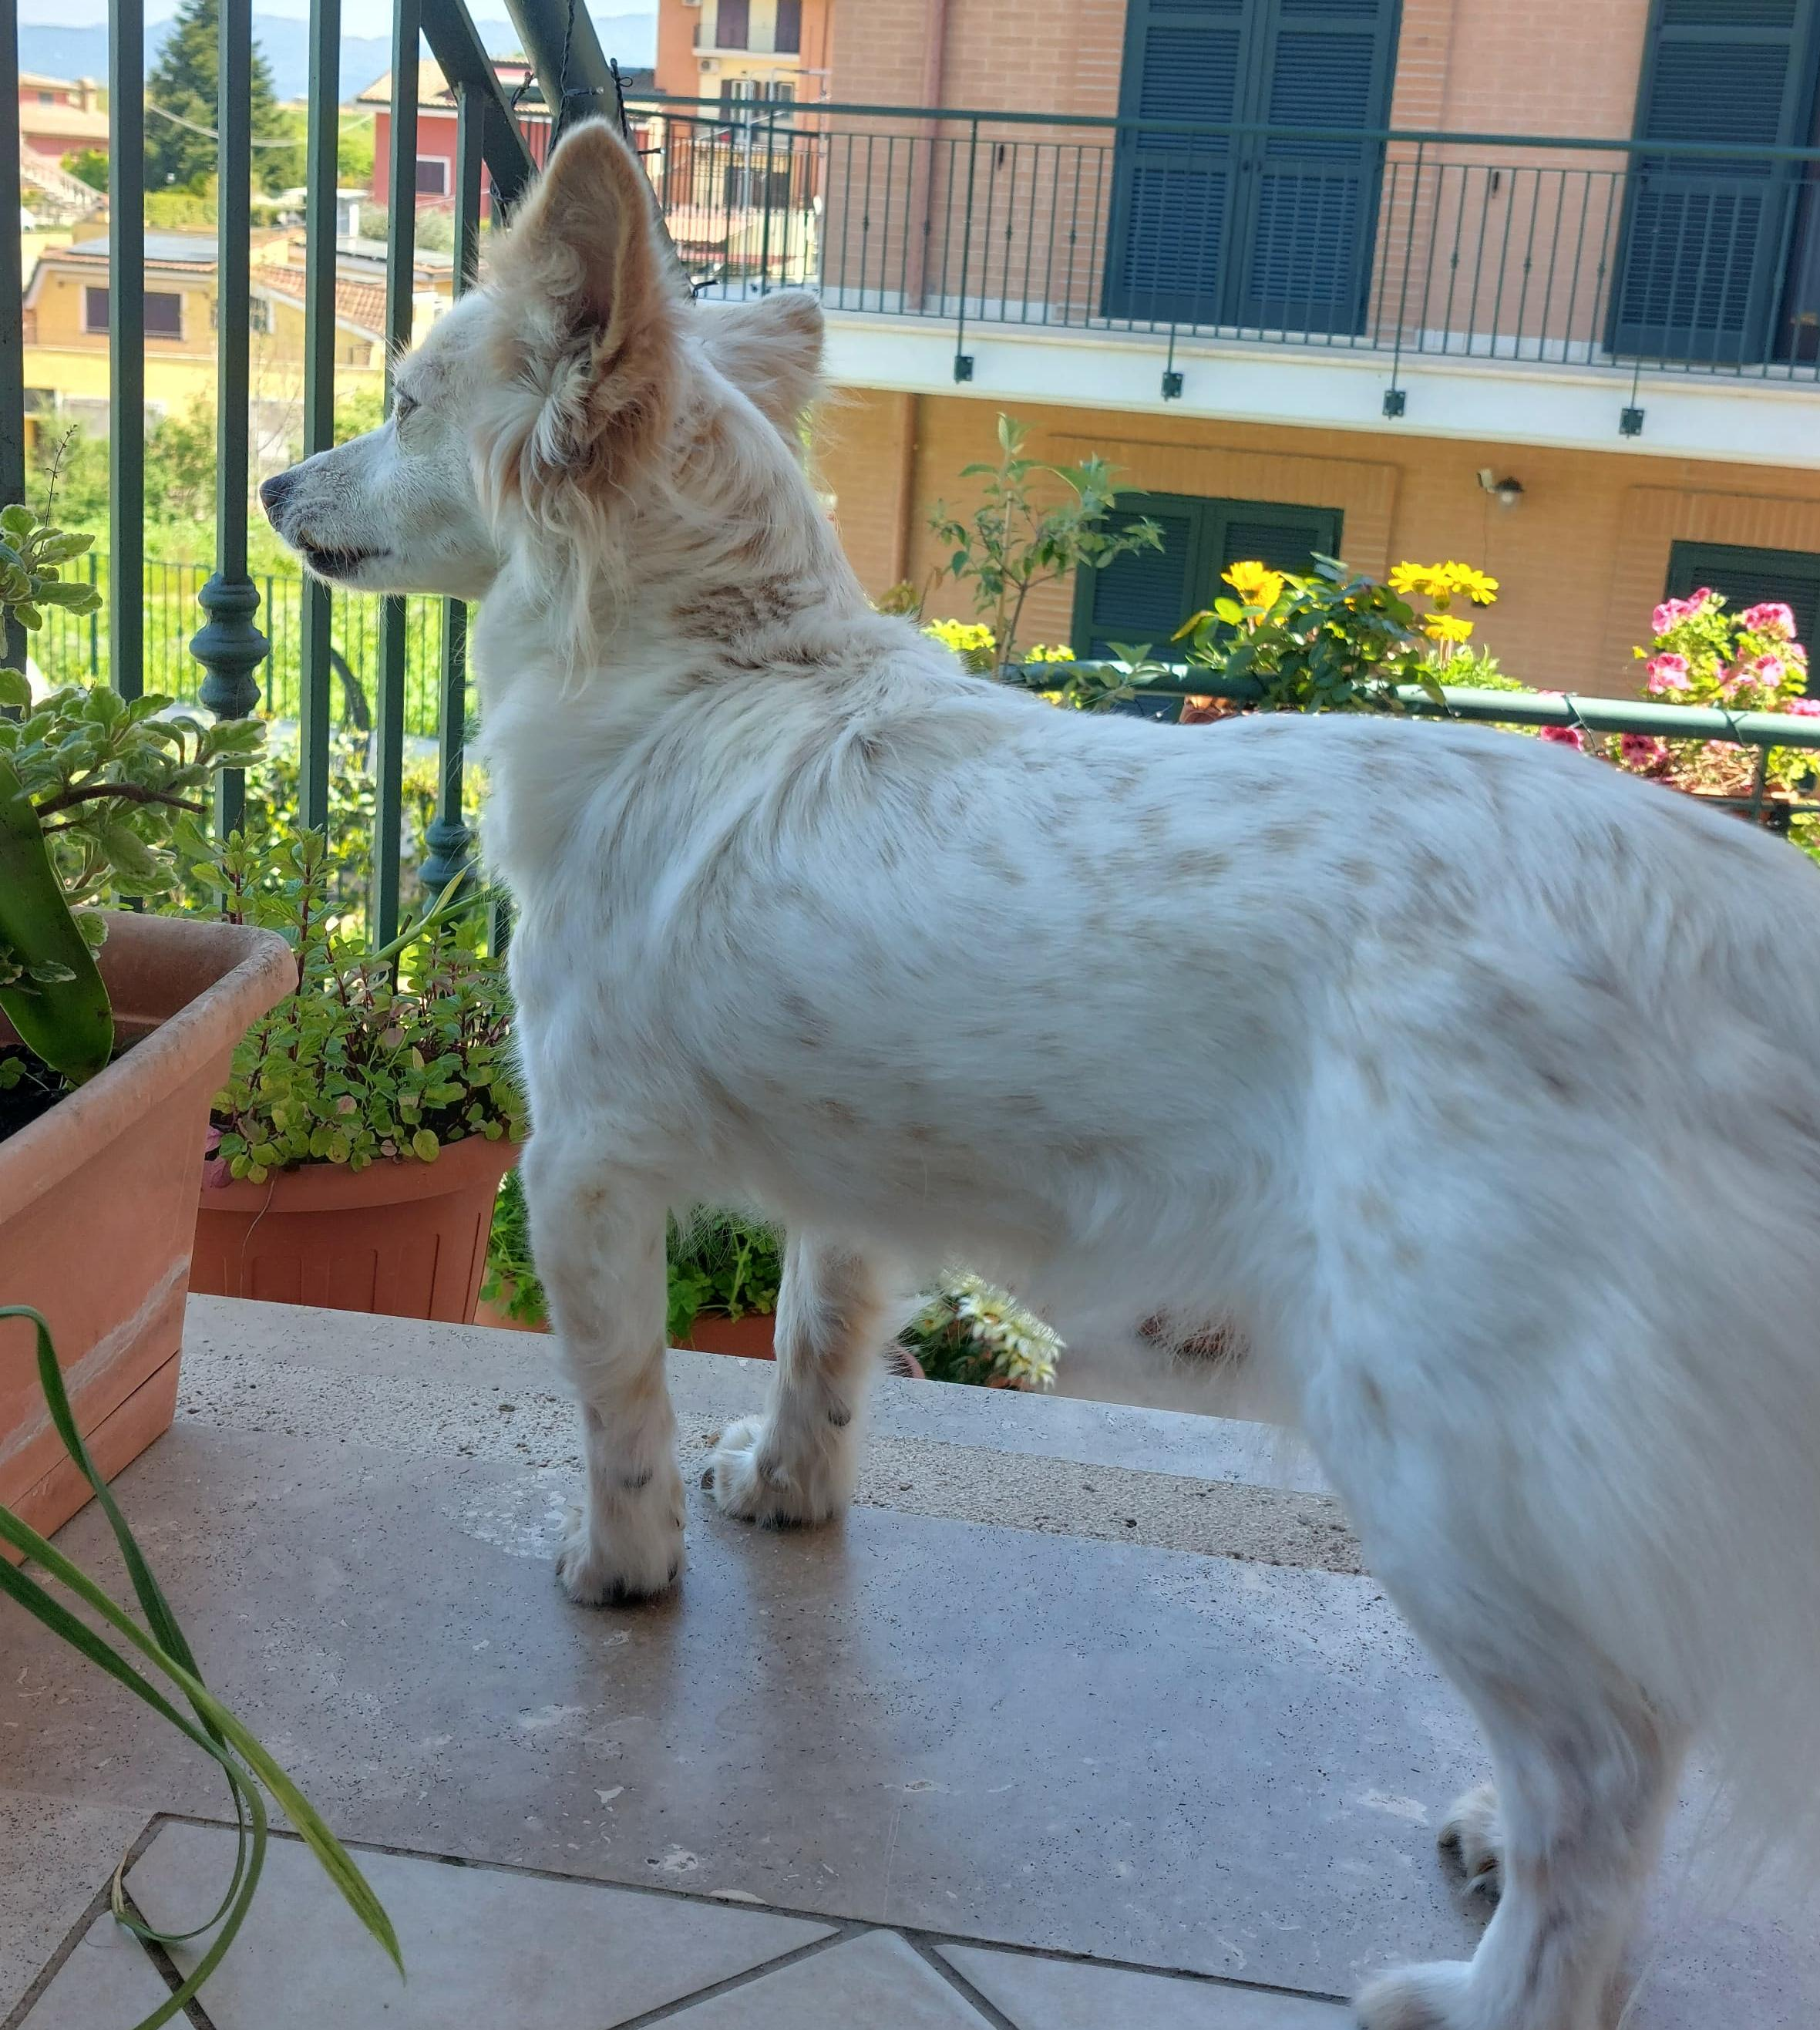
\includegraphics[width=\linewidth]{Figures/example.jpeg}
    \end{subfigure}
    \hspace{2cm}
    \begin{subfigure}[t]{0.4\linewidth}
        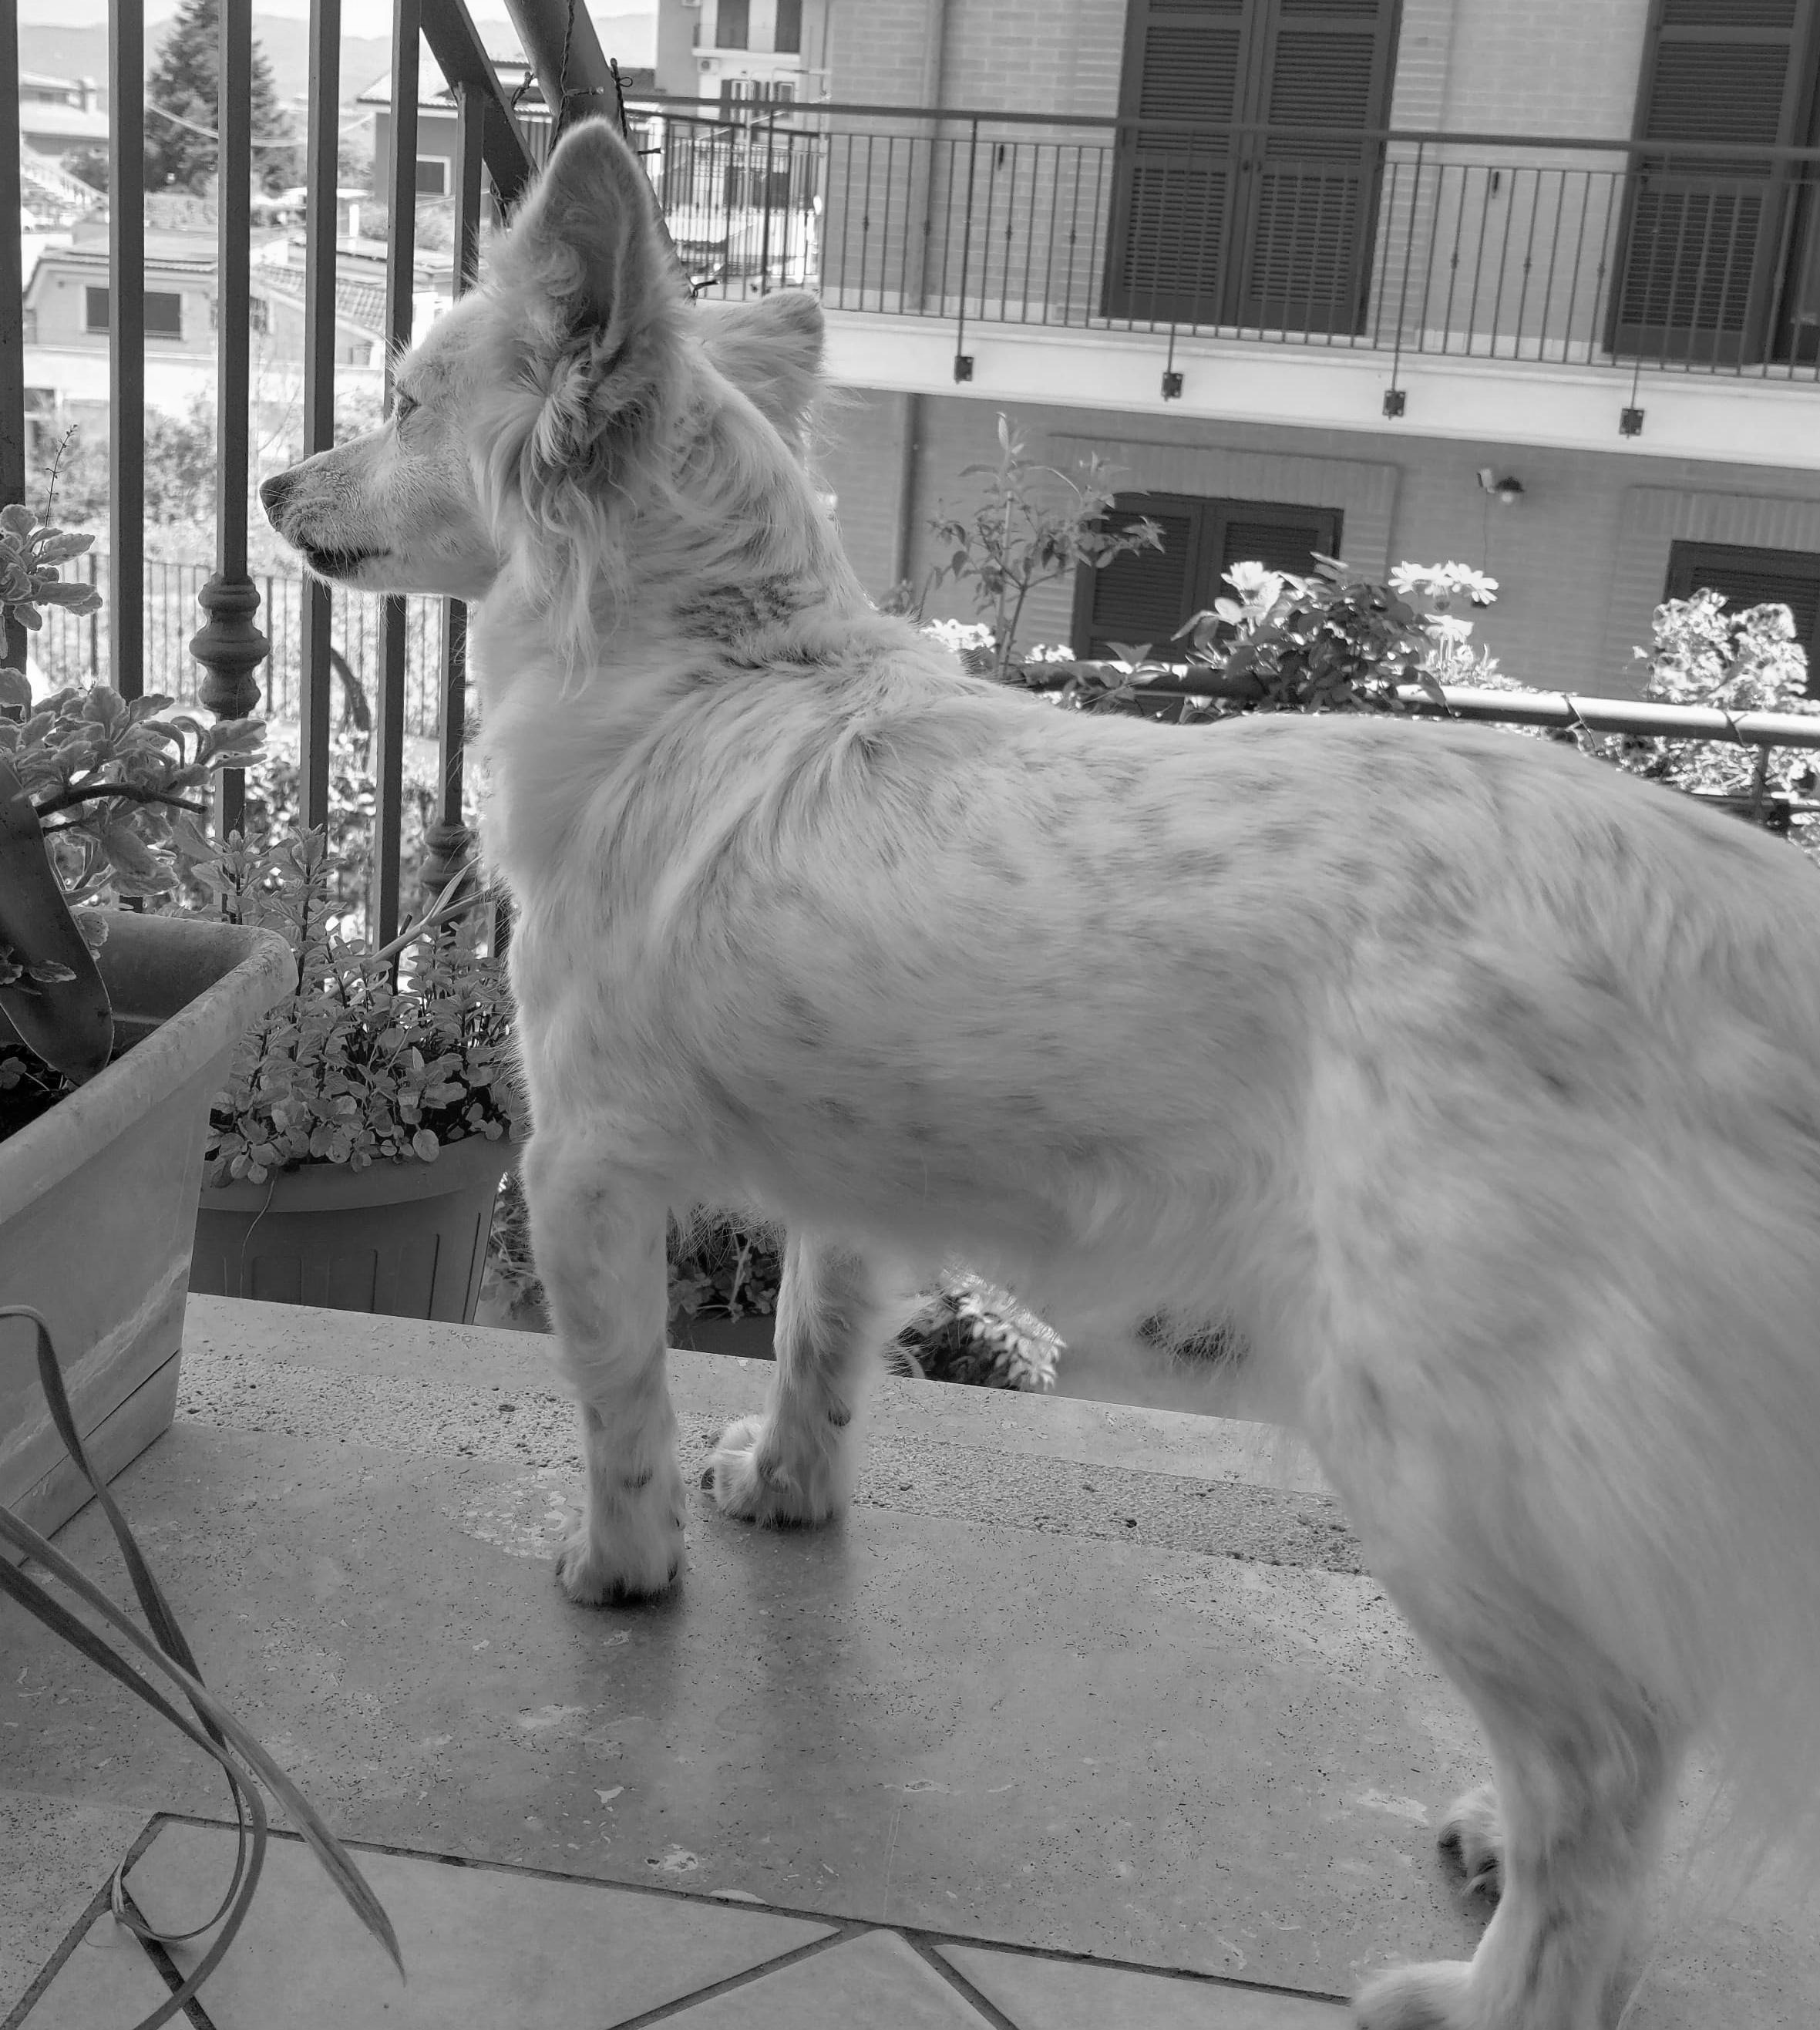
\includegraphics[width=\linewidth]{Figures/example_gray.jpeg}
    \end{subfigure}
\end{figure}
\subsection{Removing squares}
    Una delle principali sfide nell'elaborazione e raccolta del dataset riguarda la pulizia delle immagini, che possono presentare impurità significative, come la presenza di quadretti sui fogli. È essenziale rimuovere o attenuare questi elementi affinché si confondano con lo sfondo e non interferiscano con l'analisi. Inizialmente, si è considerato l'uso di tecniche statiche, come il thresholding o l'applicazione di kernel specifici per il riconoscimento dei quadretti. Tuttavia, tali tecniche rischiavano di compromettere la scrittura dell'autore cancellando dettagli. Per questo motivo, si è scelto di ricorrere a tecniche di compressione per individuare i pattern, poiché i quadretti costituiscono un pattern ben visibile e più facilmente distinguibile dalla macchina rispetto alla scrittura umana.

    \paragraph{\gls{svd}}
    Un primo test ha coinvolto l'esame dei pattern predominanti tramite una decomposizione \gls{svd}. L'immagine può essere vista come una matrice $H \times W$ di valori reali e può essere decomposta nel prodotto:
    \[
    U\Sigma V^H = M
    \]
    dove $M$ rappresenta l'immagine, $U$ e $V$ sono matrici unitarie ($UU^H = I$, stesso per $V$), $V^H$ è l'hermitiana di $V$, e $\Sigma$ è una matrice $H \times W$ con solo valori reali lungo la diagonale, chiamati valori singolari.\\
    È possibile ottenere una versione meno dettagliata di $M$ annullando alcuni valori singolari di $\Sigma$, ignorando così il contributo di determinati pattern. Si è osservato che il pattern predominante (associato al valore singolare maggiore) riguarda i quadretti, ma la sua rimozione non risolve completamente il problema, richiedendo l'eliminazione di ulteriori pattern. Il risultato ottenuto è incoraggiante, ma comporta una perdita di informazioni dalla scrittura umana, poiché anch'essa è presente tra i principali pattern identificati.

    \paragraph{\gls{fft}}
    Un'idea alternativa è effettuare un'analisi armonica delle immagini utilizzando la \gls{fft}. I quadretti si ripetono con una frequenza specifica lungo le due dimensioni del foglio e quindi si può sfruttare la loro natura regolare rispetto alla scrittura umana, che è meno ripetitiva. Così si sfrutta sia la differenza tra i pattern regolari dei quadretti e i tratti irregolari della scrittura, sia una maggiore capacità di compressione rispetto a una semplice analisi pixel per pixel.

    \noindent Per verificare questa idea, si esegue una \gls{fft} su immagini di prova: un foglio virtuale con solo quadretti e lo stesso foglio con dei disegni sopra. Nel caso del foglio senza segni, le frequenze con ampiezza maggiore si trovano principalmente allineate lungo gli assi $x$ e $y$ (\cref{fig:synthetic_grid_fft}). Aggiungendo un disegno, le frequenze principali restano pressoché le stesse (\cref{fig:synthetic_sign_fft}). Per rimuovere i quadretti, si eliminano queste frequenze significative e si ricostruisce l'immagine (\cref{fig:synthetic_clean_fft}).

    \begin{figure}
    	\centering
    	\begin{subfigure}[t]{\linewidth}
    		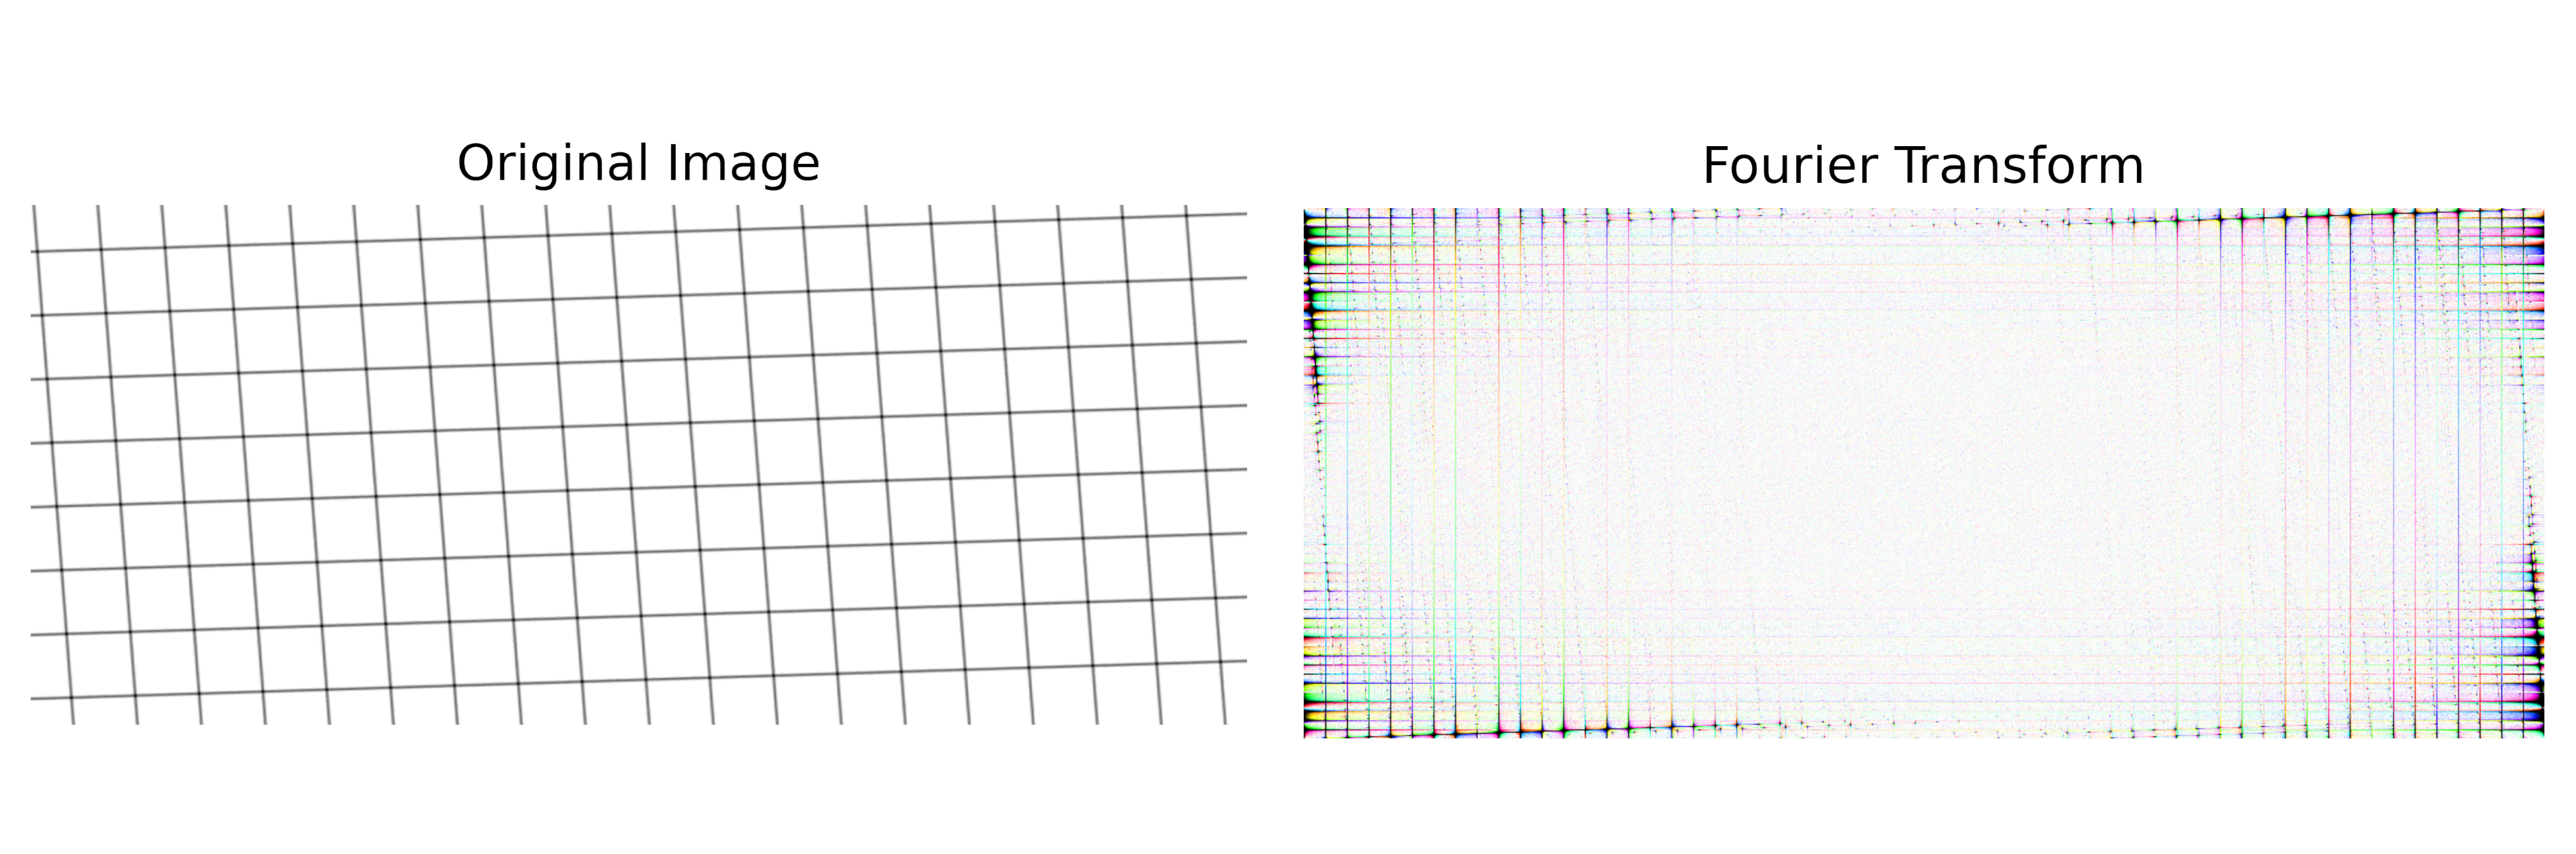
\includegraphics[width=\linewidth]{Figures/grid_fft.png} \caption{Un reticolato lievemente trasformato, causato da una scansione imperfetta. Le frequenze più significative sono evidenziate in nero.} \label{fig:synthetic_grid_fft}
    	\end{subfigure}
    	\begin{subfigure}[t]{\linewidth}
    		\includegraphics[width=\linewidth]{Figures/test_fft.png} \caption{Un reticolato deformato con una scritta sovrapposta. Le frequenze del reticolato restano visibili.} \label{fig:synthetic_sign_fft}
    	\end{subfigure} \begin{subfigure}[t]{\linewidth}
    		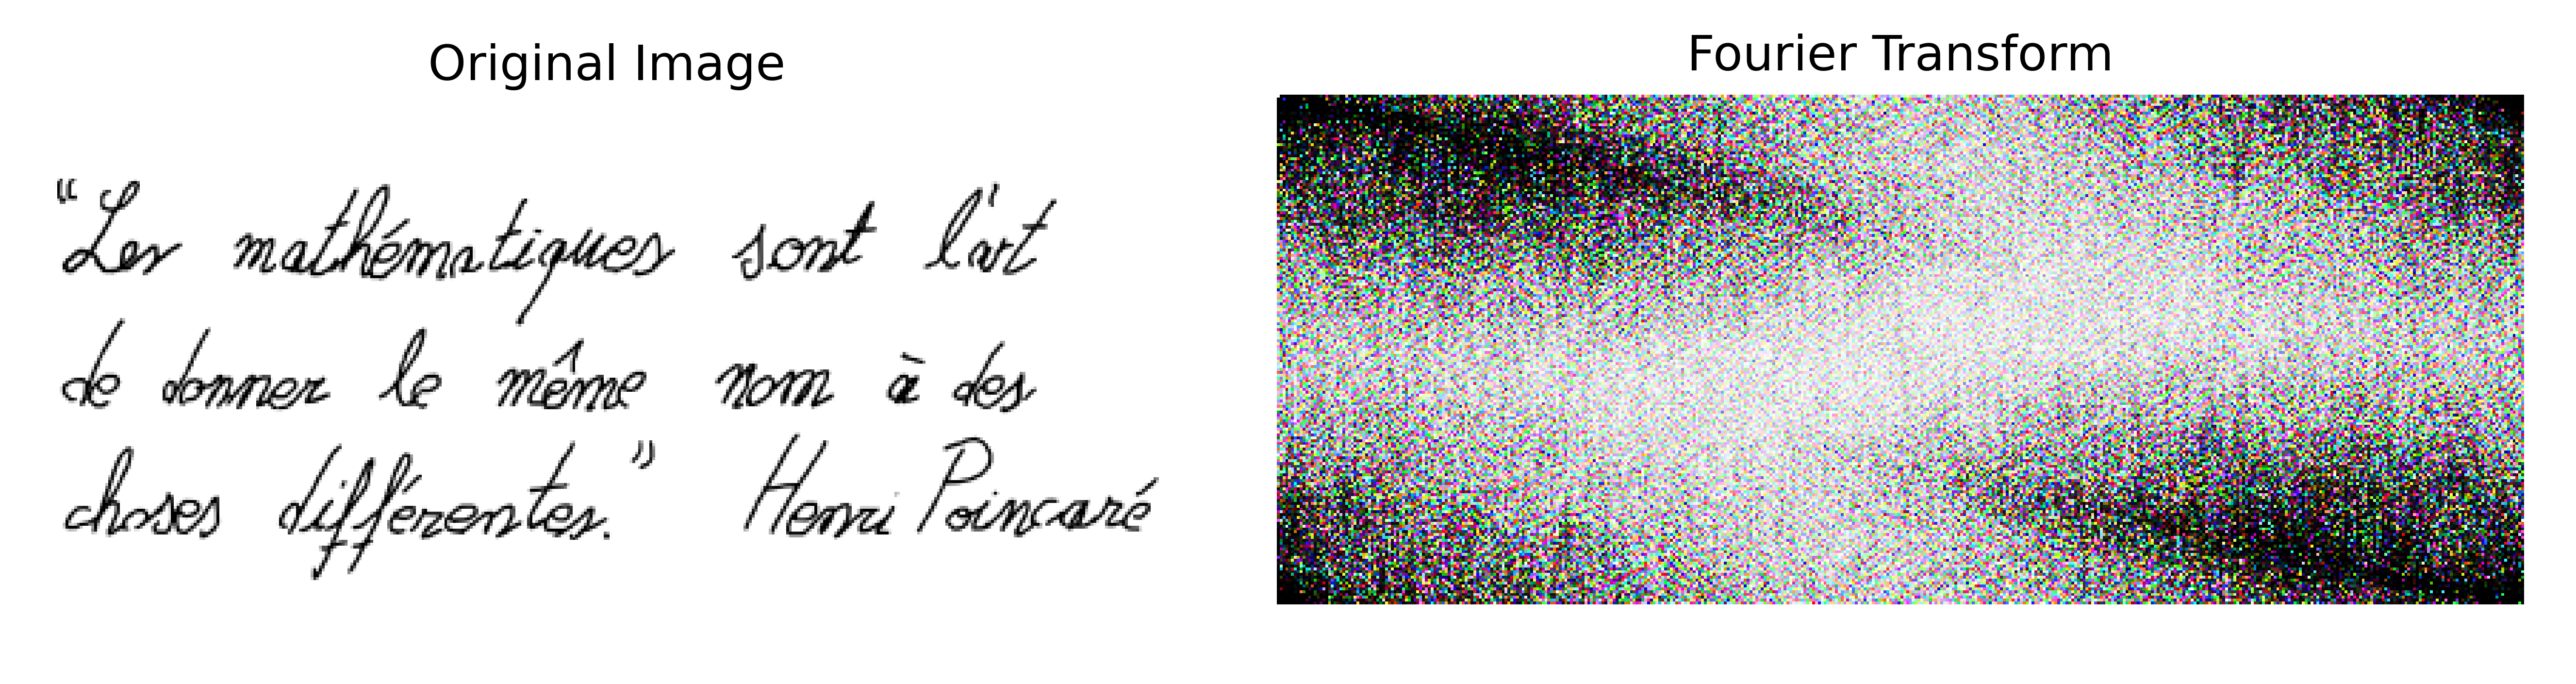
\includegraphics[width=\linewidth]{Figures/clean_fft.png} \caption{La scritta senza reticolo non mostra coefficienti di Fourier significativi, poiché mancano pattern ricorrenti.} \label{fig:synthetic_clean_fft}
    	\end{subfigure}
    	\caption[Synthetic FFT test]{Coefficiente di Fourier dell'immagine bidimensionale. I quadretti mostrano coefficienti di Fourier simili a quelli delle onde quadre: $\text{sqwave}(t) = \frac{4}{\pi}\sum_{k=1}^{\infty}\frac{\sin\left(2\pi(2k-1)t\right)}{2k-1}$. Le intensità più significative sono a intervalli regolari con intensità decrescenti.}
    \end{figure}

    \noindent Empiricamente, analizzando $10$ immagini reali selezionate casualmente, si è osservato che i quadretti sono stati rimossi con successo senza danneggiare le scritte, annullando le ampiezze corrispondenti al primo $0.05$ percentile delle frequenze più significative.

    \noindent Tuttavia, questa operazione distorce parzialmente i colori. Infatti, in un'immagine originale, la distribuzione dei livelli di grigio è piuttosto intuitiva: la maggior parte dei pixel è bianca, mentre solo una piccola percentuale è composta da tonalità di grigio più scure. Dopo la ricostruzione, si nota la presenza di molte tonalità di grigio intermedie, che interessano sia lo sfondo che le scritte.

    \noindent Si è osservato che, nelle immagini originali, i pixel con un livello di grigio inferiore a $0.2$ appartengono certamente alle scritte, mentre quelli con un livello di grigio superiore a $0.8$ corrispondono allo sfondo bianco della pagina. Di conseguenza, si contano i pixel delle scritte e dello sfondo bianco nell'immagine originale. Nell'immagine ripulita, i pixel più scuri (con un valore di grigio inferiore a $0.2$ nell'immagine originale) vengono assegnati al nero, mentre i pixel più chiari (con un valore di grigio superiore a $0.8$ nell'immagine originale) vengono assegnati al bianco.

    \noindent Questo processo viene realizzato tramite una "normalizzazione con morsetto": i colori vengono espansi in modo tale che i pixel che devono essere neri assumano un valore di grigio inferiore a $0$, mentre i pixel bianchi superano il valore di $1$. Successivamente, si imposta a $0$ qualsiasi valore negativo e a $1$ qualsiasi valore maggiore di $1$. Un risultato di questa procedura è mostrato in \cref{fig:first_reconstruct}

    \begin{algorithm}[h]
    	\caption[Cleaning procedure using FFT]{Cleaning procedure using FFT.\\
    		\begin{minipage}[t]{\linewidth}
    			\textsc{INPUT}
    			\begin{itemize}[noitemsep, topsep=0pt]
    				\item[$\mathcal{I}$:] Image as matrix $W\times H$ in gray scale
    				\item[$p$:] percentile of significant magnitudes
    				\item[$a$:] thresholds $(\min, \max)$
    			\end{itemize}
    			\textsc{OUTPUT} $\mathcal{I}_{\text{new}}$: Image as matrix $W\times H$ in gray scale
    		\end{minipage}
    	}
    	\begin{algorithmic}[1]
    		\Procedure{CleanFFT}{$\mathcal{I}, p, a$}
    		\State $\hat{\mathcal{I}} \gets \text{normalize}\left(\mathcal{I}\right)$
    		\State $F_{\hat{\mathcal{I}}} \gets \text{fft2d}\left(\hat{\mathcal{I}}\right)$
    		\State $f = (f_1, \dots, f_{W\times H}) \gets \text{argsort}\left(\text{flatten}\left(F_{\hat{\mathcal{I}}}\right), \text{rule=abs}\right)$
    		\State $f_{\text{best}} \gets f\left[\text{last}\; \lfloor{p\cdot\text{length}\rfloor}\;\text{values}\right]$ \Comment{components with high magnitude}
    		\For{$k \in f_{\text{best}}$}
    			\State $F_{\hat{\mathcal{I}}}[k] = 0.0$
    		\EndFor
    		\State $\hat{\mathcal{I}} \gets \text{ifft2d}\left(F_{\hat{\mathcal{I}}}\right)$ \Comment{rebuild normalized image}
    		\State $w_{\text{cnt}} \gets \textbf{count}\;\mathcal{I} \geq a(\max)$ \Comment{normalization using dilation and clamp}
    		\State $b_{\text{cnt}} \gets \textbf{count}\;\mathcal{I} \leq a(\max)$
    		\State $h_{w} \gets \max_{w_{\text{cnt}}^{\mathrm{-th}}}\mathcal{\hat{I}}$
    		\State $h_{w} \gets \min_{b_{\text{cnt}}^{\mathrm{-th}}}\mathcal{\hat{I}}$
    		\State $\mathcal{I}_{\text{new}} \gets \frac{\mathcal{\hat{I}} - h_{b}}{h_{w}-h_{b}}$
    		\Where{$\mathcal{I}_{\text{new}} > 1$, $\mathcal{I}_{\text{new}} = 1$}
    		\Where{$\mathcal{I}_{\text{new}} < 0$, $\mathcal{I}_{\text{new}} = 0$}
    		\State \Return $\mathcal{I}_{\text{new}}$
    		\EndProcedure
    	\end{algorithmic}
    	\label{alg:CleaningFFT}
    \end{algorithm}
